This chapter describes how the use of the different datasets were implemented.

\section{Folkehelseinstituttet}
The data contained two different sets, and it was a simple job to plot them in a graph. Figure \ref{fig:infstat} show the three last seasons of influenza. The plotting was done manually as fhi only provides the data in pdf format.

\begin{figure}[ht]
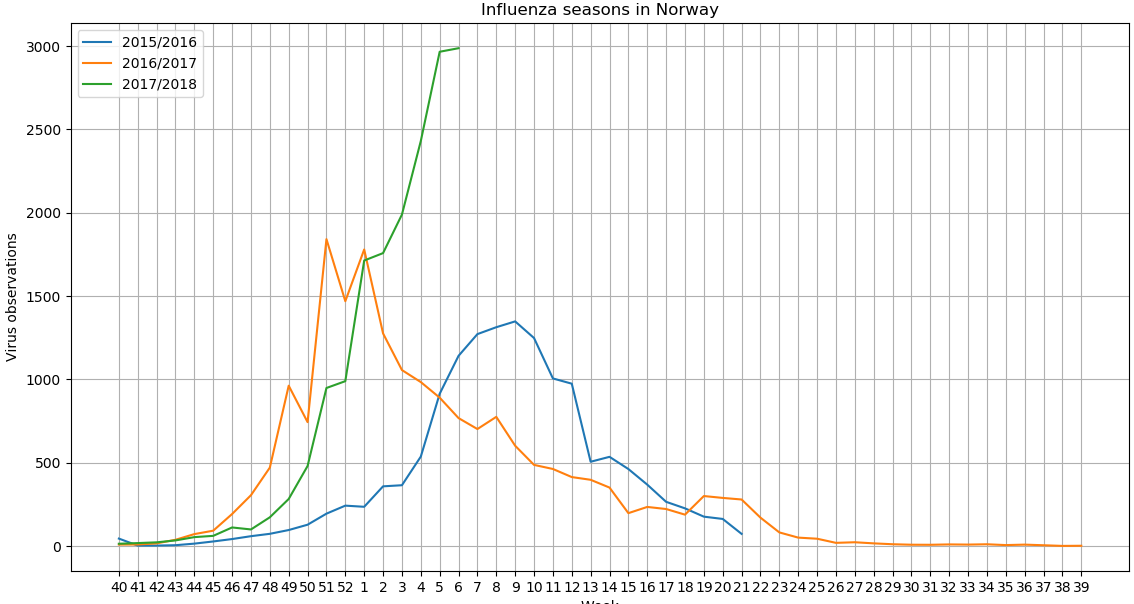
\includegraphics[width=16cm]{influenza_15_till_18}
\centering
\caption{Influenza seasons}
\label{fig:infstat}
\end{figure}

Figure \ref{fig:ilsstat} shows the ILS of the year 2016/2017. This was not done manually as data was provided in a simple .xlsx file 

\begin{figure}[ht]
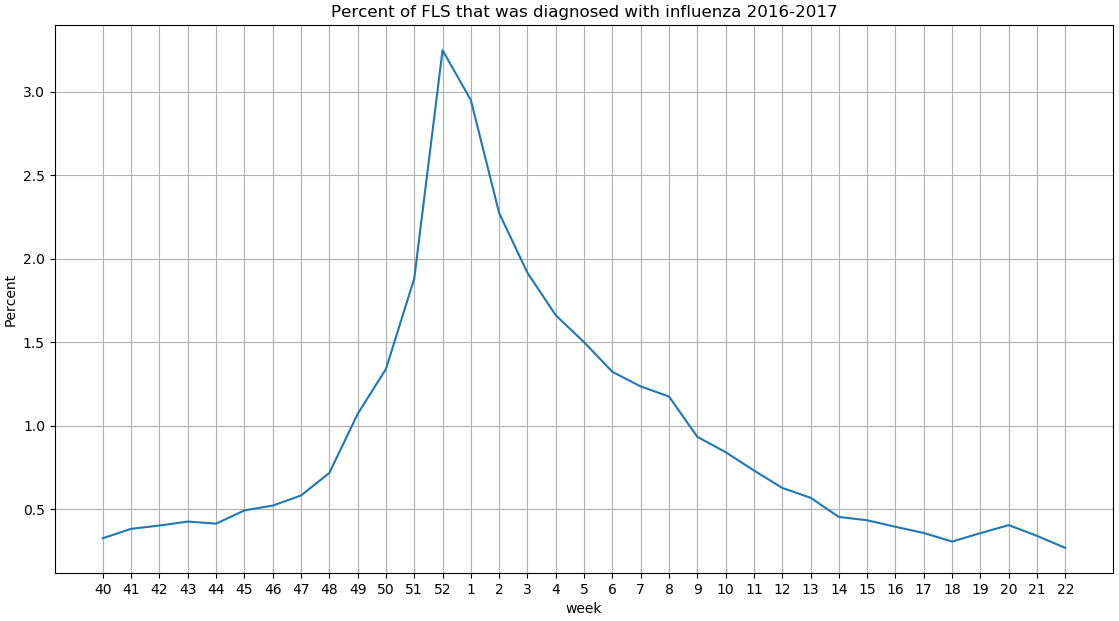
\includegraphics[width=16cm]{ILS_16_till_17}
\centering
\caption{Influenza like symptoms season 2016/2017}
\label{fig:ilsstat}
\end{figure}

\newpage

\section{Vegvesenet}
From the XML statistics some simple graphs were created in python showing the total annual traffic on Norwegian roads from 2002 to 2015 as seen in figure \ref{fig:anualtotal}. 

\begin{figure}[ht]
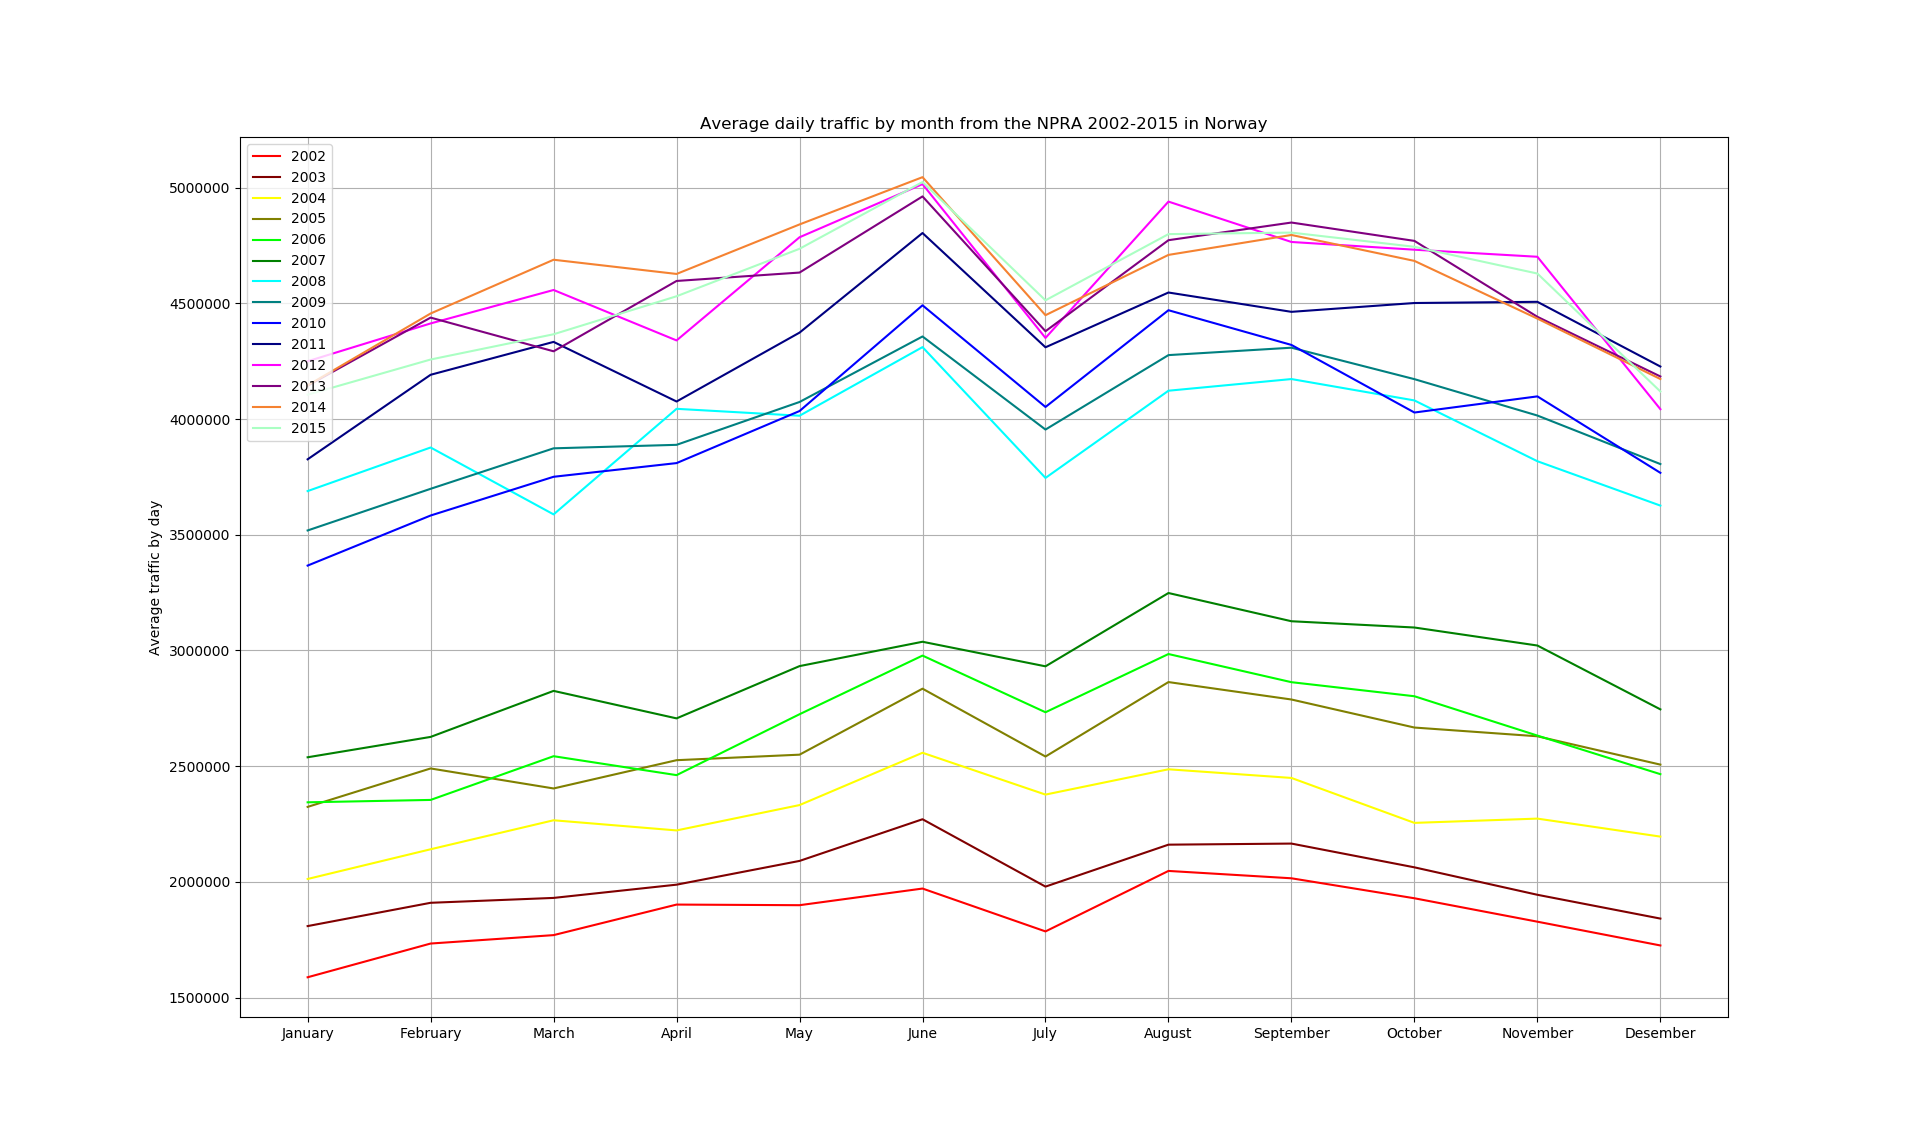
\includegraphics[width=16cm]{xml_02_15_annual_total}
\centering
\caption{Annual traffic 2002-2015}
\label{fig:anualtotal}
\end{figure}

Also derived from this the annual traffic of the two cities Bergen and Oslo, which are towns in interest. Figure \ref{fig:anualbergen} shows the traffic in Bergen, and figure \ref{fig:anualoslo} show the traffic in Oslo.

\begin{figure}[ht]
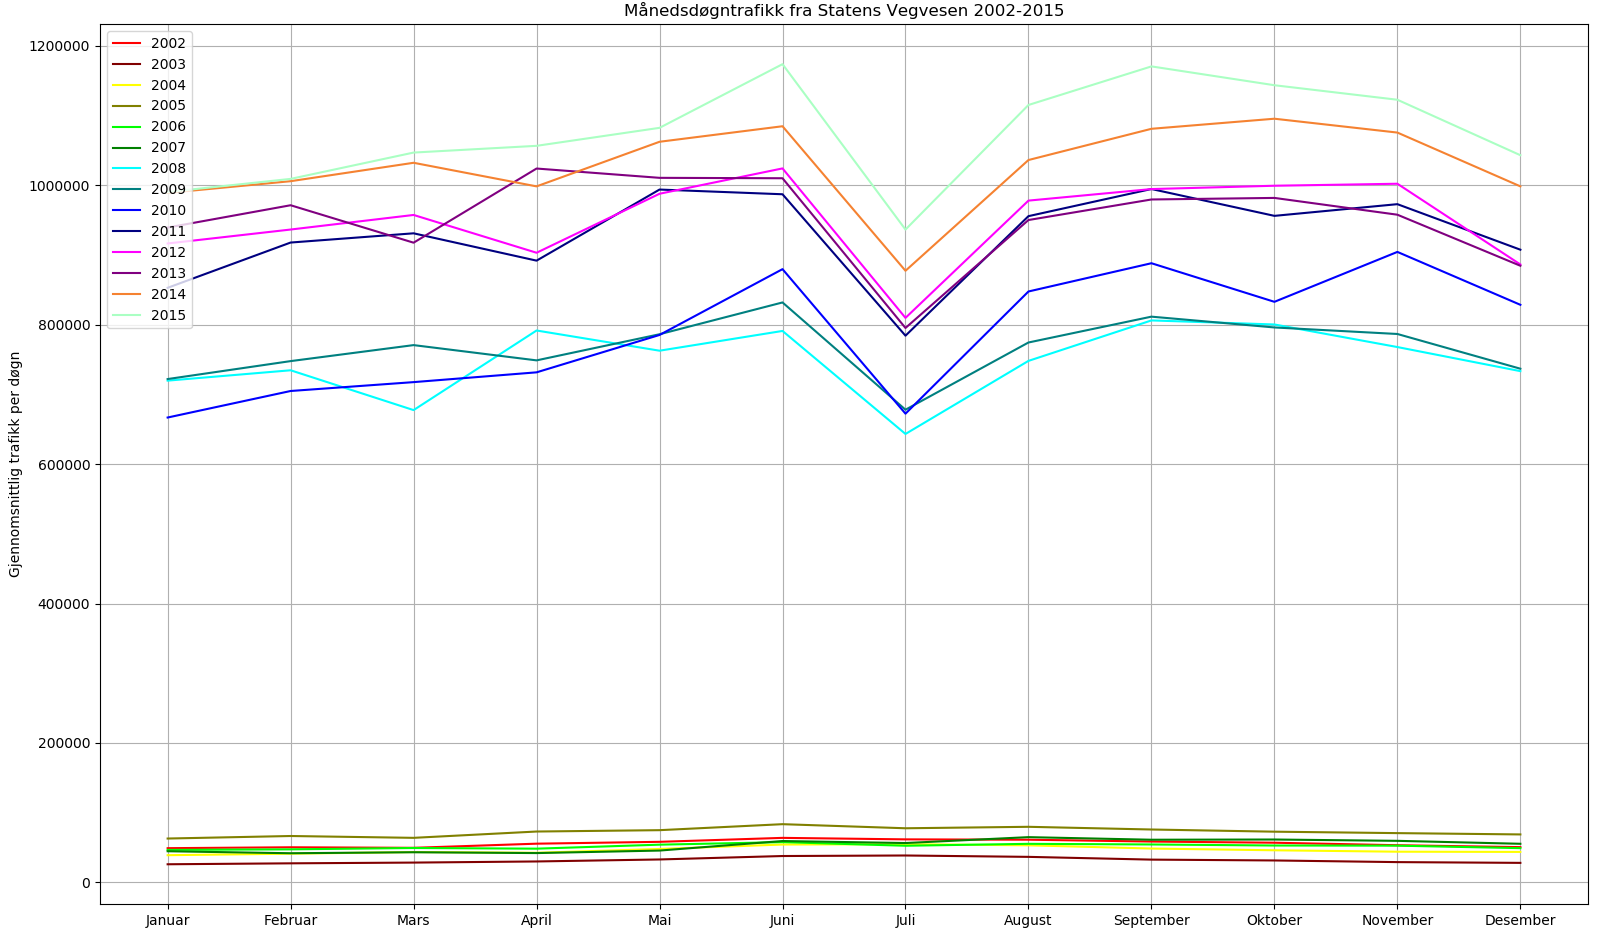
\includegraphics[width=16cm]{xml_02_15_annual_bergen}
\centering
\caption{Bergen traffic 2002-2015}
\label{fig:anualbergen}
\end{figure}

\begin{figure}[ht]
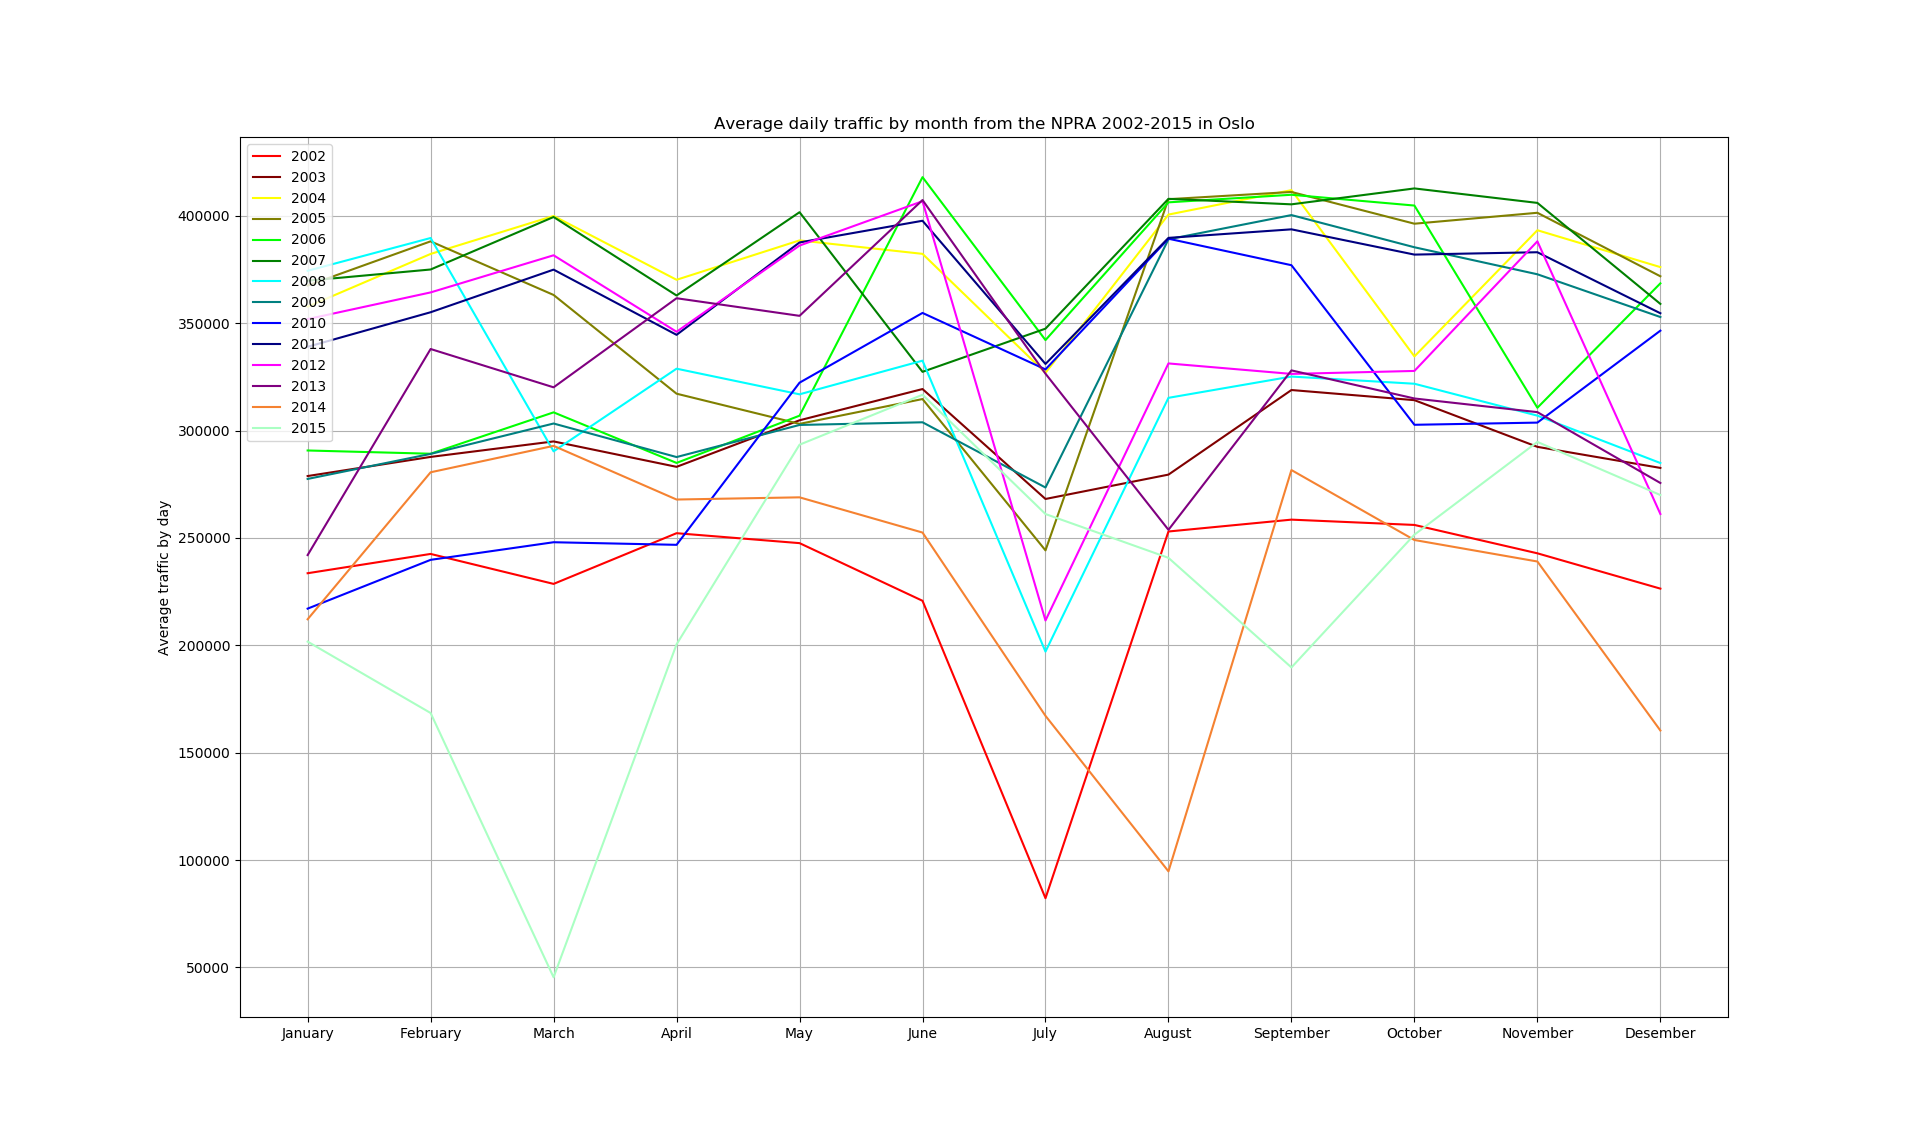
\includegraphics[width=16cm]{xml_02_15_annual_oslo}
\centering
\caption{Oslo traffic 2002-2015}
\label{fig:anualoslo}
\end{figure}
The dataset is an XLM file structure that is downloaded from the NPRA manually. A python program was created that reads through all rows and collects the relevant columns into an array and then draws a graph. For the annual graph every month of every year was collected. For the towns of Bergen and Oslo the correct roads were identified and loaded from a separate text file, then every year of every month of those roads were collected, loaded into an array and the drawn as a graph. The separate text file is to make it easy to edit should these roads change in the future.
The problem of using these datasets is that the data is an average calculation of monthly traffic, this is too coarse for comparison against the influenza data as they are on a weekly basis. Luckily upon further investigation and help from the NPRA better data was accessible upon request, hidden from that available on their website. A set of traffic registration stations was needed to define the temporal bounds of each area of interest. Defined are the towns of Oslo and Bergen, as well as the whole of Norway on a level 1 basis. The level 1 registrations ensures continually registration throughout the year, and is exactly what this project requires.

Figures \ref{fig:weeklybergen}, \ref{fig:weeklyoslo} and \ref{fig:weeklystavanger} shows the traffic on a weekly basis. This provides a better resolution for better analysis.
\begin{figure}[ht]
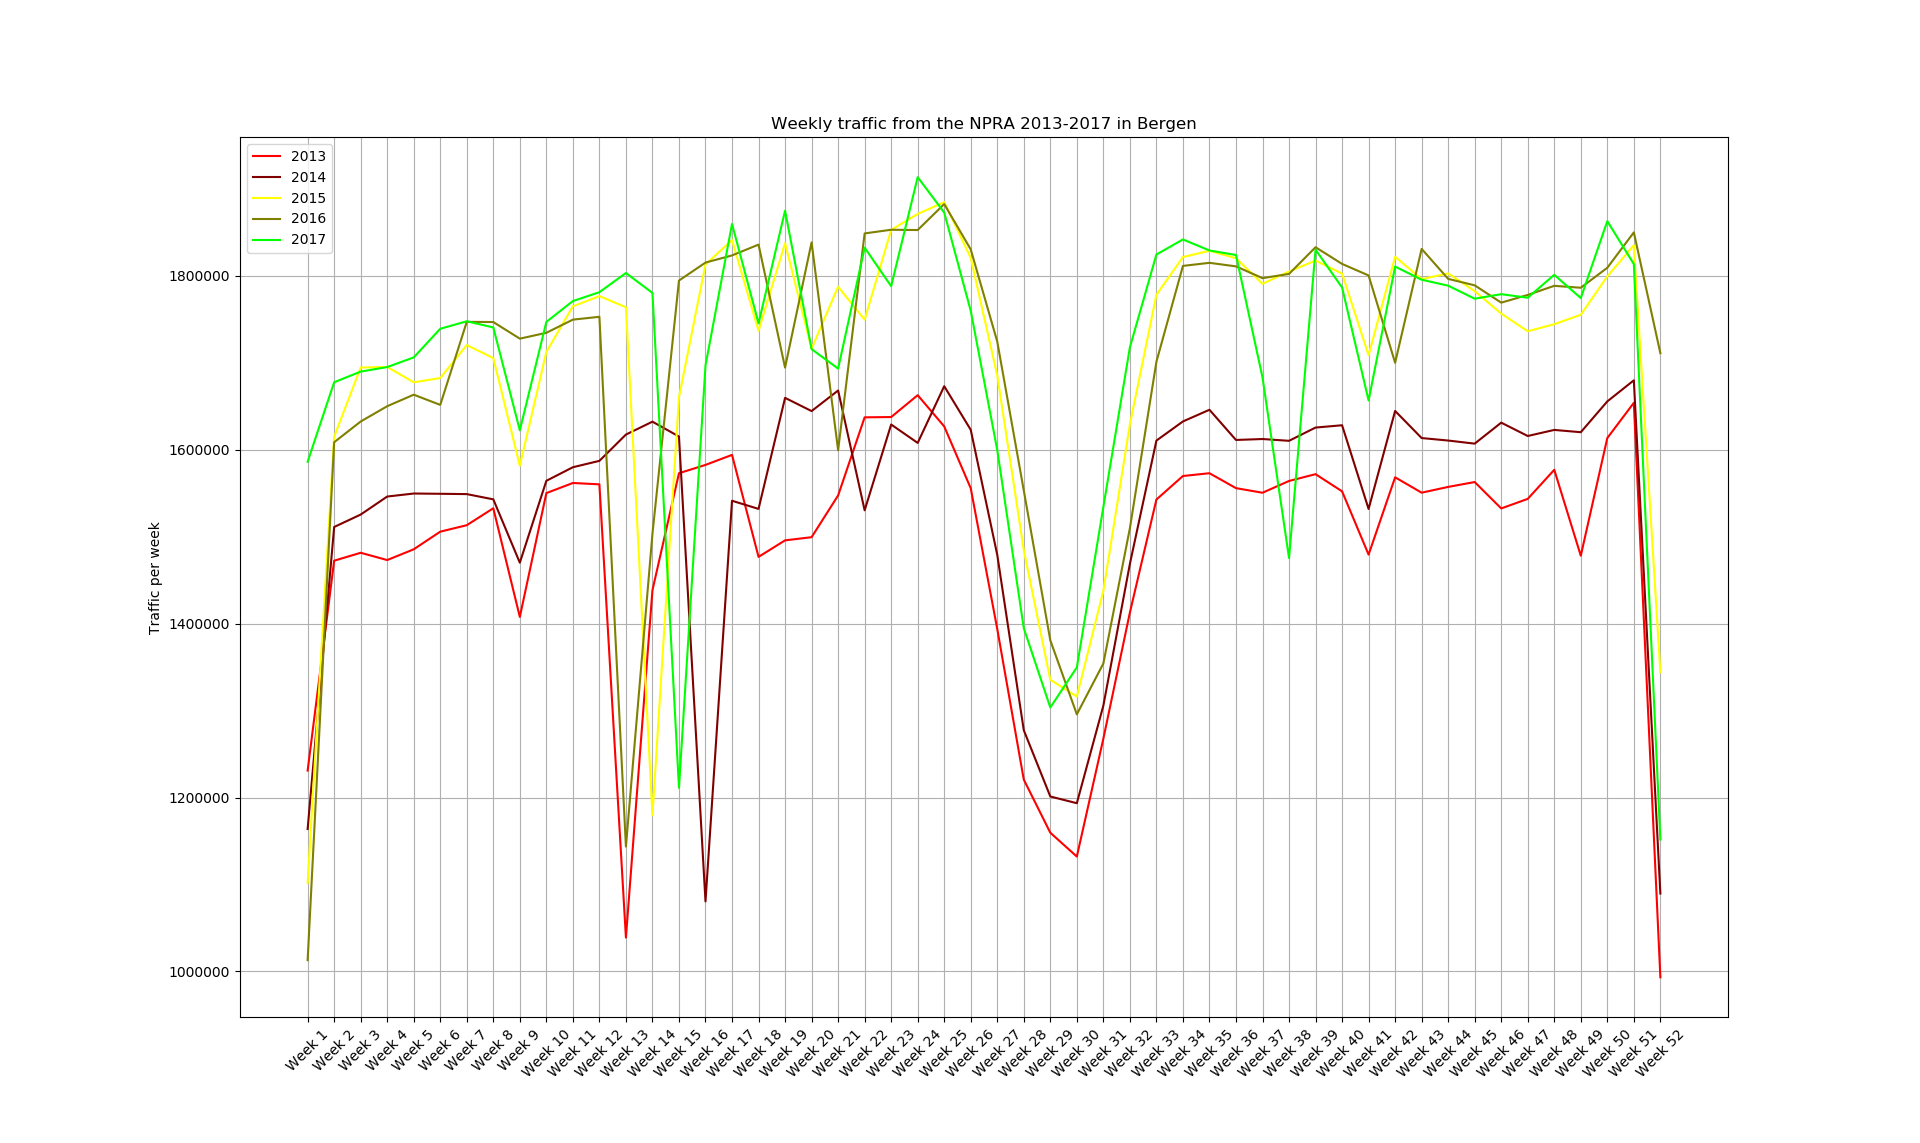
\includegraphics[width=16cm]{NPRA_13_17_weekly_bergen}
\centering
\caption{Weekly data of the city of Bergen}
\label{fig:weeklybergen}
\end{figure}

\begin{figure}[ht]
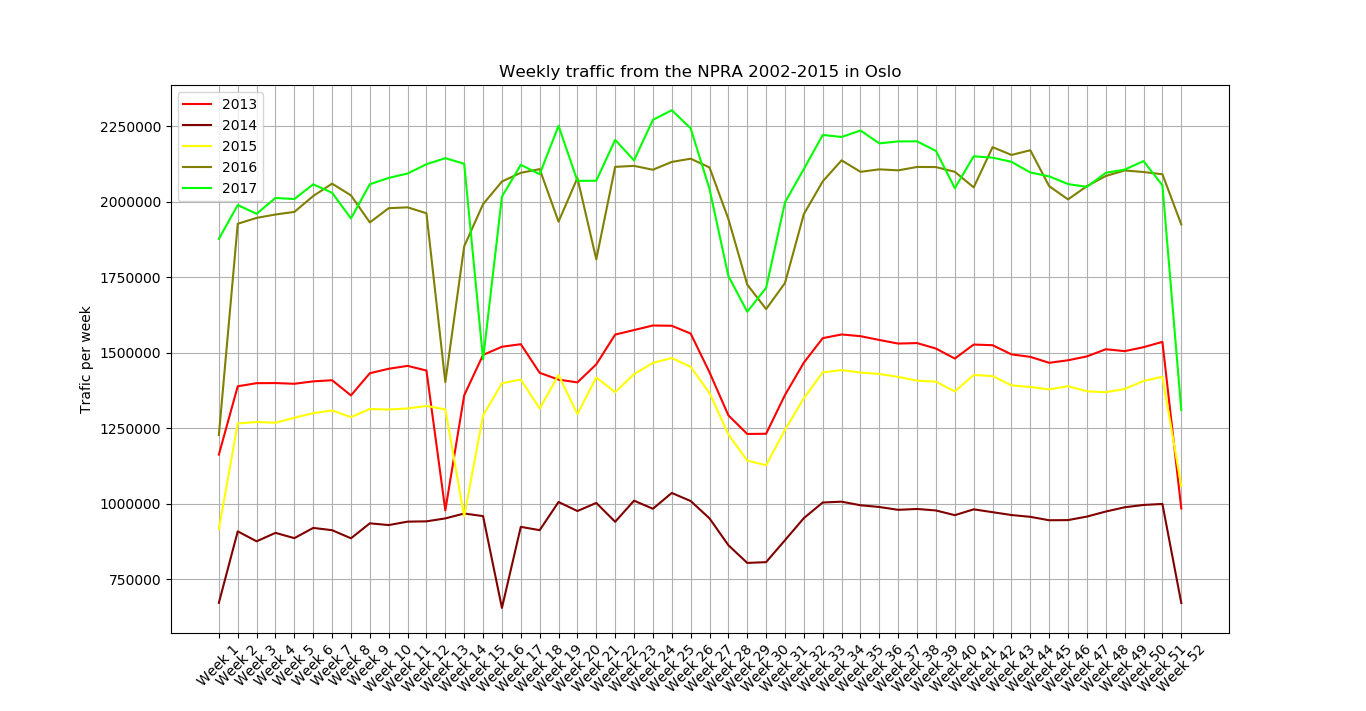
\includegraphics[width=16cm]{NPRA_13_17_weekly_oslo}
\centering
\caption{Weekly data of the city of Oslo}
\label{fig:weeklyoslo}
\end{figure}

\begin{figure}[ht]
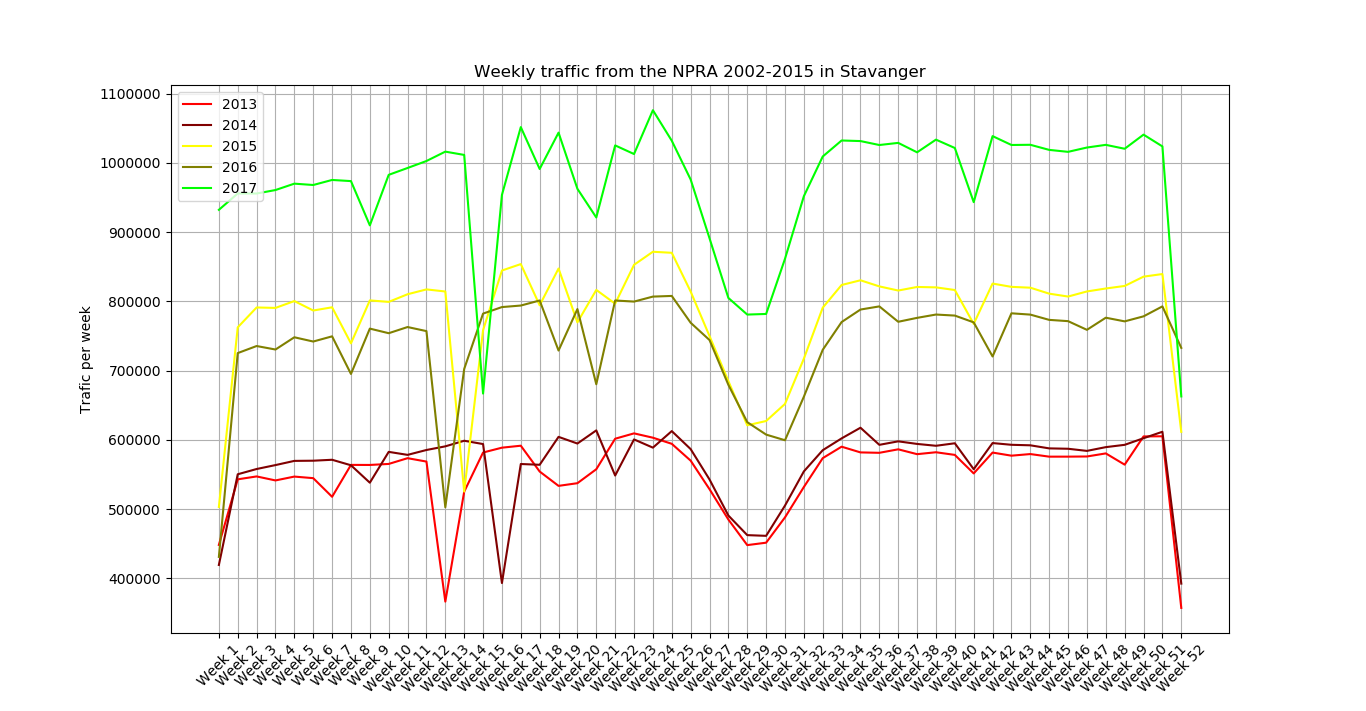
\includegraphics[width=16cm]{NPRA_13_17_weekly_stavanger}
\centering
\caption{Weekly data of the city of Stavanger}
\label{fig:weeklystavanger}
\end{figure}

Figure \ref{fig:boundsbergen}, \ref{fig:boundsoslo} and \ref{fig:boundsstavanger} shows the different geospatial bounds used to define the cities. The green cirlces with numbers inside show where and how many traffic registration stations there are.

\begin{figure}[ht]
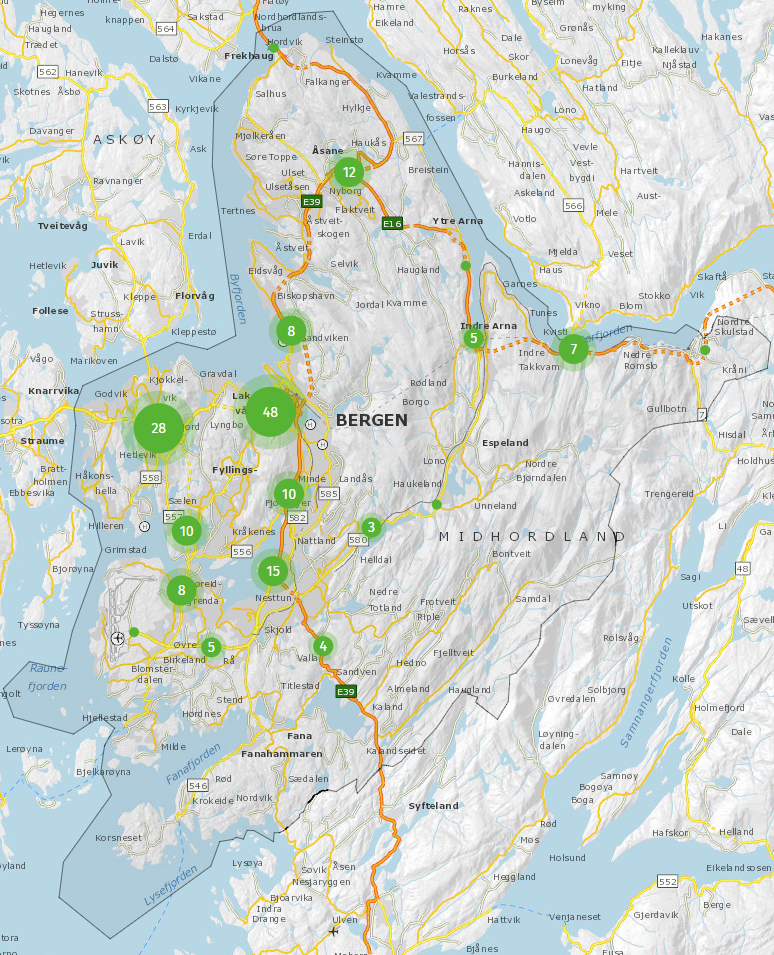
\includegraphics[width=16cm]{nivaa_1_bergen}
\centering
\caption{Geospatial bounds of Bergen}
\label{fig:boundsbergen}
\end{figure}

\begin{figure}[ht]
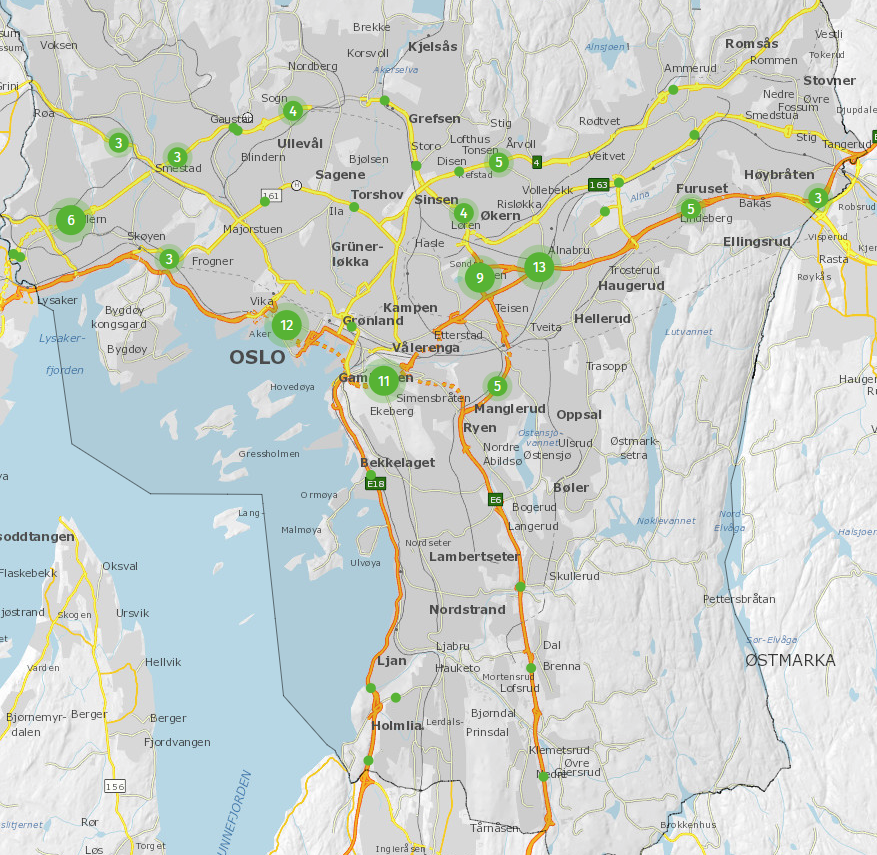
\includegraphics[width=16cm]{nivaa_1_oslo}
\centering
\caption{Geospatial bounds of Oslo}
\label{fig:boundsoslo}
\end{figure}

\begin{figure}[ht]
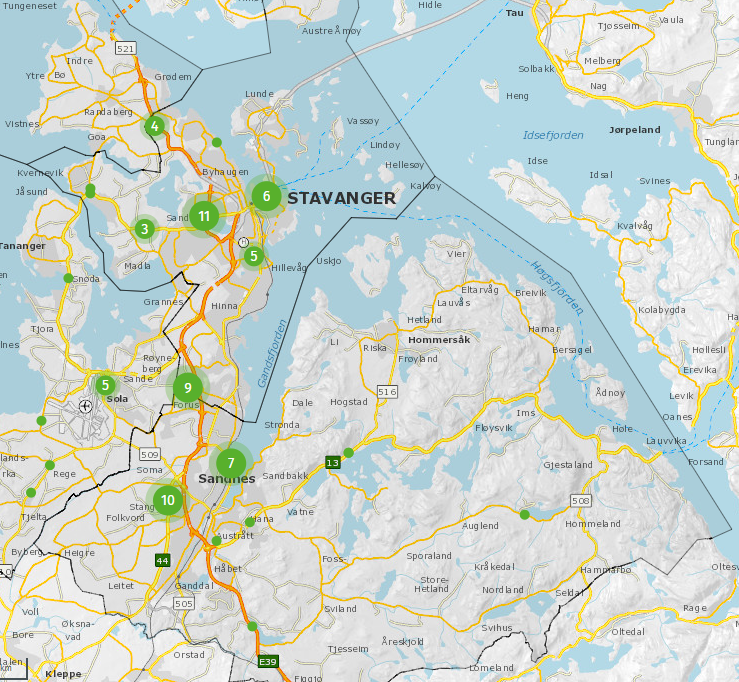
\includegraphics[width=16cm]{nivaa_1_stavanger}
\centering
\caption{Geospatial bounds of Stavanger}
\label{fig:boundsstavanger}
\end{figure}

\newpage\newpage

\section{Twitter}
Using the REST search API it was paramount that in order to build a sufficient dataset acquiring and collecting data had to begin as soon as possible. A simple python program was created that takes the input of the API keys and the keywords to be searched upon . The program ensures that no duplicate messages are recorded, and the limit of a hundred tweets was overcome simply by searching for yet another hundred from the last date of the previous hundred, until the date limit was reached.
The output is appended to a file in this format: id, date, location, tweet.

Analysis of the output then need to be divided into categories based on relevant content.

\section{Kolumbus}